\documentclass[11pt]{report}
\usepackage[margin=2.3cm]{geometry}
\usepackage[fleqn]{amsmath}
\usepackage{nccmath}
\usepackage{alltt}
\usepackage{sectsty}
\usepackage{titlesec}
\newcommand{\ts}{\textsuperscript}
\usepackage{graphicx}
\graphicspath{ {../images/} }
\usepackage{subfig}
\usepackage[hidelinks]{hyperref}
\newcommand{\linespace}{\vspace{0.3cm}\noindent}
\renewcommand{\bibname}{References}

\titlespacing*{\section}{0pt}{0.8\baselineskip}{0.2\baselineskip}

\begin{document}

\begin{titlepage}
    \begin{center}
        \vspace*{1cm}
        
        \textbf{CO3093 COURSEWORK 2 - Report}
        
        \vspace{0.5cm}
		Big Data \& Predictive Analytics - Classification \& Clustering
        
        \vspace{1.5cm}
        
        \textbf{Ihtasham Chaudhry}
        
        \vfill
        
        \vspace{0.8cm}
                
        Department of Informatics\\
        University of Leicester\\
        28\ts{th} March 2018
        
    \end{center}
\end{titlepage}

\newpage

\section{Exploring the data}

\linespace
In this section we will explore the data-set \texttt{Diabetes 130-US hospitals for years 1999-2008}. 

\subsection{Exploring the data as a whole}

To visualise and explore the data-set it's important to extract key-information as some of the columns in the data-set are not key in analysing the data.

\linespace
Firstly, we must remove any rows/columns that have missing values and that we may not be able to use in order to conduct any further experiments or analysis on. There seem to be many rows with \texttt{?} values, i.e. unknown values and mostly on the columns \texttt{weight} and \texttt{payer\_code}. So we can remove these as they will not be relevant in either clustering or analysing the data-set.

\linespace
From the numerical data we can make the following analyses:

\begin{itemize}
	\item The mean time spent in hospital by a patient who has been admitted is approximately 4 days. 
	\item The mean number of procedures each patient has received is 1.34 procedures. The median being 1, which shows that number of procedures are skewed towards smaller values (positive skew). To visualise this we can see Figure 1.
	\item The number of diagnoses per patient has a mean of 7.4 diagnoses per patient. Also in this case we observe that the values are skewed towards smaller values and to illustrate this we can look at Figure 2. 
\end{itemize}

\begin{figure}[ht]
	\begin{minipage}[b]{.5\textwidth}
	\centering
	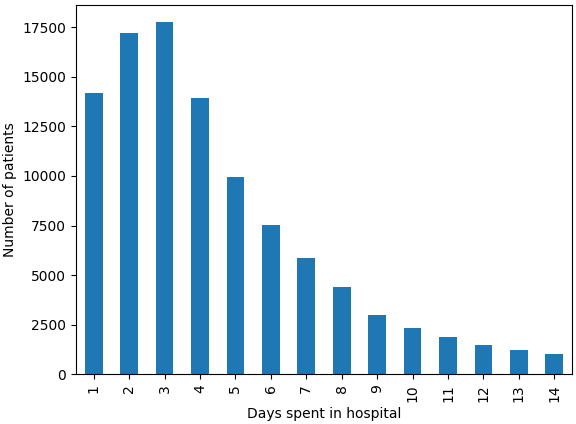
\includegraphics[width=1\textwidth]{tih_hist.png}
	\caption{Days spent in hospital per patient}
	\end{minipage}
	\hfill
	\begin{minipage}[b]{.5\textwidth}
	\centering
	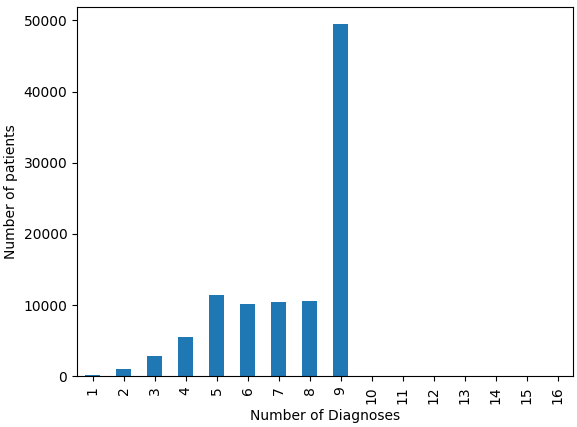
\includegraphics[width=1\textwidth]{nod_bar.png}
\caption{Diagnoses per patient}
\end{minipage}
\end{figure}

\noindent
From Figure 1 we can observe that most patients stay in the hospital between 1 and 4 days, from this we can also see that there is positive skewness. Furthermore, from Figure 2 we can observe that most patients have 9 diagnoses (almost 50\% of patients), however there are many patients that have less than 9 and rarely any patients that exceed 9 number of diagnoses. This shows that most patients had 9 diagnoses which may include diseases, injuries or any other symptom that was entered onto the system \cite{table2}. We can also make a confident assertion that a higher number of diagnoses will result in higher chance of a patient being readmitted to the hospital due to the nature of these diagnoses. It may directly correlate to the probability of readmissions.

\clearpage
\linespace
At a basic level we can visualise the distribution of diabetic patients by race and gender, the results of this can be seen below.

\begin{figure}[ht]
	\begin{minipage}[b]{.5\textwidth}
	\centering
	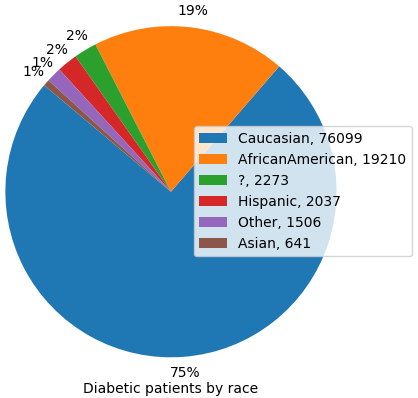
\includegraphics[width=1\textwidth]{race_pie.png}
	\caption{Proportion of diabetics by race}
	\end{minipage}
	\hfill
	\begin{minipage}[b]{.5\textwidth}
	\centering
	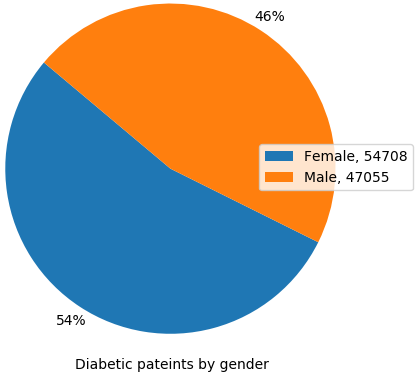
\includegraphics[width=1\textwidth]{gender_pie.png}
\caption{Proportion of diabetics by gender}
\end{minipage}
\end{figure}

\linespace
From this we can see that majority of diabetic patients admitted to US hospitals from 1999 to 2008 are mostly Caucasian (75\%). By analysing the gender split, it's almost equal split however a higher percentage of females (54\%) than males (46\%). By looking at the ethnicity and gender features, we can confidently make the assertion that it does not motivate whether or not a patient is likely to be readmitted to the hospital. It does not provide us with any information as to whether a Caucasian male is more likely to be readmitted for diabetes than a African America female, for example. This it may not be useful to consider these features in our model for predicting whether a patient will be readmitted. 


  \begin{thebibliography}{1}

  \bibitem{table2} Beata Strack, Jonathan P. DeShazo, Chris Gennings, et al., “Impact of HbA1c Measurement on Hospital Readmission Rates: Analysis of 70,000 Clinical Database Patient Records,” BioMed Research International, vol. 2014, Article ID 781670, 11 pages, 2014. doi:10.1155/2014/781670 - \url{https://www.hindawi.com/journals/bmri/2014/781670/cta/} - Table found at: \url{https://www.hindawi.com/journals/bmri/2014/781670/tab2/}

  \end{thebibliography}

\end{document}